\begin{frame}
\frametitle{Introduction to the Normal Distribution}
\begin{itemize}
\item
Recall the experiment whereby a die was rolled 100 times, and the sum of the 100 values was recorded.
\item
This experiment was repeated a very large number of times (e.g. 100,000 times ) in a simulation study.
\item
A histogram was drawn to depict the distribution of outcomes of this experiment.
\item Recall that we agreed that ``bell-shaped" was a good description of the histogram.

\end{itemize}
\end{frame}


\frame{
\frametitle{Normal Distribution}

\begin{center}
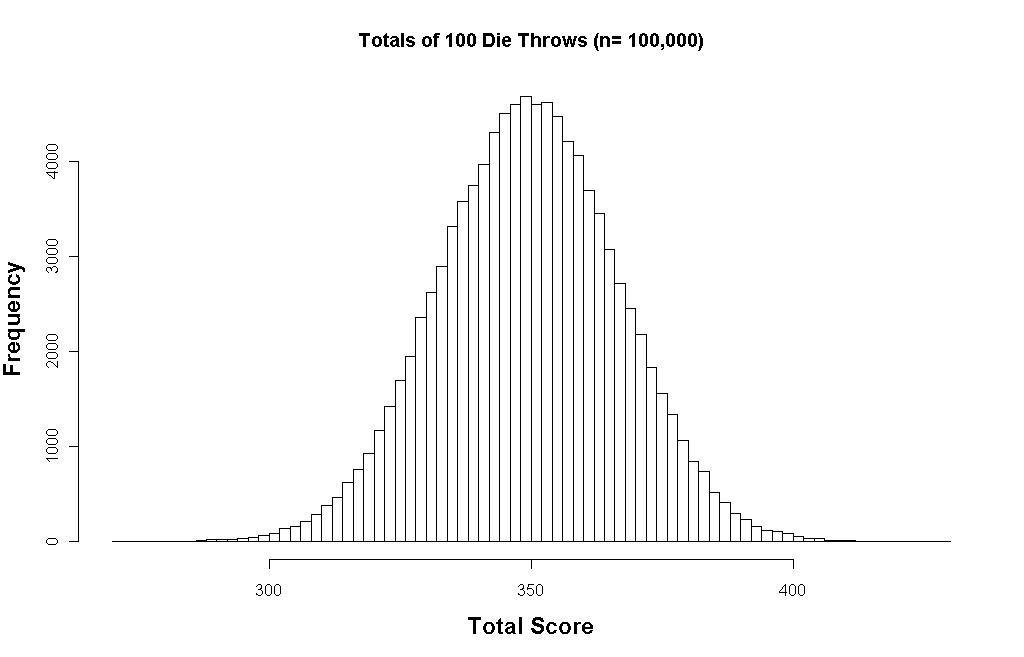
\includegraphics[scale=0.30]{images/3aDieHist3}
\end{center}

}



\frame{
\frametitle{Normal Distribution} 
\begin{itemize}
\item Normal distributions are a family of distributions that have the same general shape. 
\item They are symmetric with scores more concentrated in the middle than in the tails. Normal distributions are sometimes described as bell shaped. 
\item Examples of normal distributions are shown below. Notice that they differ in how spread out they are. The area under each curve is the same. 
\item The height of a normal distribution can be specified mathematically in terms of two parameters: the mean ($\mu$) and the standard deviation ($\sigma$). 

\end{itemize}
}

\frame{
\frametitle{Normal Distribution}
\begin{itemize}
\item The normal distribution is perhaps the most widely used distribution for a random variable.
\item Normal distributions have the same general shape: the bell curve.
\item They are symmetric with scores more concentrated in the middle than in the tails.
%\item Examples of normal distributions are shown below. Notice that they differ in how spread out they are. The area under each curve is the same.
\item The height of a normal distribution can be defined mathematically in terms of two fundamental parameters: the mean ($\mu$) and the standard deviation ($\sigma$).
\item A normally distributed random variable X is denoted $ X \sim \mbox{N} (\mu, \sigma^2)$ (note that we use the variance term here)
    \item The mean and standard deviation are vital for calculating probabilities.
\end{itemize}
}
%------------------------------------------------------------------------%
\frame{
\frametitle{The Normal Distribution}
The \textbf{\emph{probability density function}} of the normal distribution is given as
\[ f(x) = \frac{1}{\sqrt{2\pi\sigma^2}} e^{ -\frac{(x-\mu)^2}{2\sigma^2} } \]

Integrating this formula would allow us to compute probabilities.
However, we will not use this formula, although we later discuss what a probability density function is.
}

\frame{
\frametitle{Normal Distribution}

\begin{center}
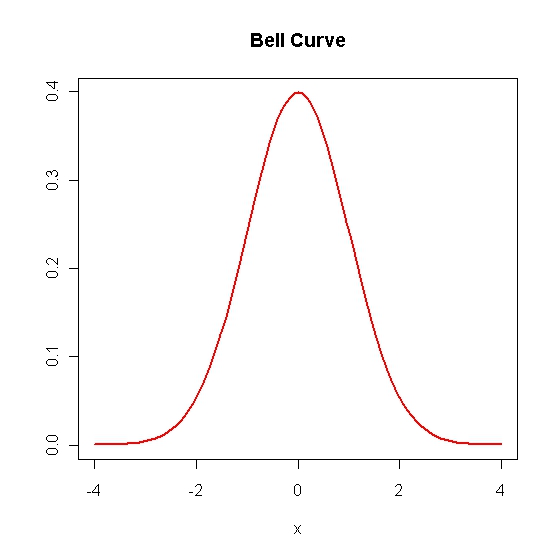
\includegraphics[scale=0.30]{images/5ABellCurve}
\end{center}

}
%------------------------------------------------------------------%
\frame{
\frametitle{ Characteristics of the Normal probability distribution}
\begin{itemize}
\item[1] The highest point on the normal curve is at the mean, which is also the median and mode of the distribution.
\item[2] \alert{[VERY IMPORTANT]}
The normal probability curve is bell-shaped and symmetric, with the shape of the curve to the left of the mean a mirror image of the shape of the curve to the right of the mean.
\item[3] The standard deviation determines the width of the curve. Larger values of the the standard deviation result in wider flatter curves, showing more dispersion in data.
\item[4] The total area under the curve for the normal probability distribution is 1.
\end{itemize}
}
%------------------------------------------------------------------%
\frame{
\frametitle{ Characteristics of the Normal probability distribution}
\begin{itemize}
\item The interval defined by \textbf{the mean} $ \pm 1 \times $ standard deviation includes $68\%$ of the observations ,leaving $16\%$ (approx) in each tail.
\item The interval defined by \textbf{the mean} $ \pm 1.96 \times $ standard deviation includes $95\%$ of the observations ,leaving $2.5\%$ (approx) in each tail.
\item The interval defined by \textbf{the mean} $ \pm 2.58 \times $ standard deviation includes $99\%$ of the observations ,leaving $0.5\%$ (approx) in each tail.
\end{itemize}
\textbf{Remark:} It is useful to know this numbers, but we will do all calculations from first principles.
}

%------------------------------------------------%
\frame{
\frametitle{Normal Distribution}
The standard normal distribution is a normal distribution with a mean of 0 and a standard deviation of 1. 
Normal distributions can be transformed to standard normal distributions by the formula:
\[ Z = {X - \mu \over \sigma} \]
where X is a score from the original normal distribution, $\mu$ is the mean of the original normal distribution, and $\sigma$ is the standard deviation 
of original normal distribution. The standard normal distribution is sometimes called the Z distribution. 
A z score always reflects the number of standard deviations above or below the mean a particular score is. 
For instance, if a person scored a 68 on a test with a mean of 50 and a standard deviation of 9, then they scored 2 standard deviations above the mean. 
Converting the test scores to z scores, an X of 70 would be:
\[ Z = {68 - 50 \over 9} \]
So, a Z score of 2 means the original score was 2 standard deviations above the mean. Note that the z distribution will only be a normal distribution if the original distribution (X) is normal. 
 
}



